\newpage
\subsection{Caso d'uso UC9: Acquisto API}
\label{UC9}
\begin{figure}[ht]
	\centering
	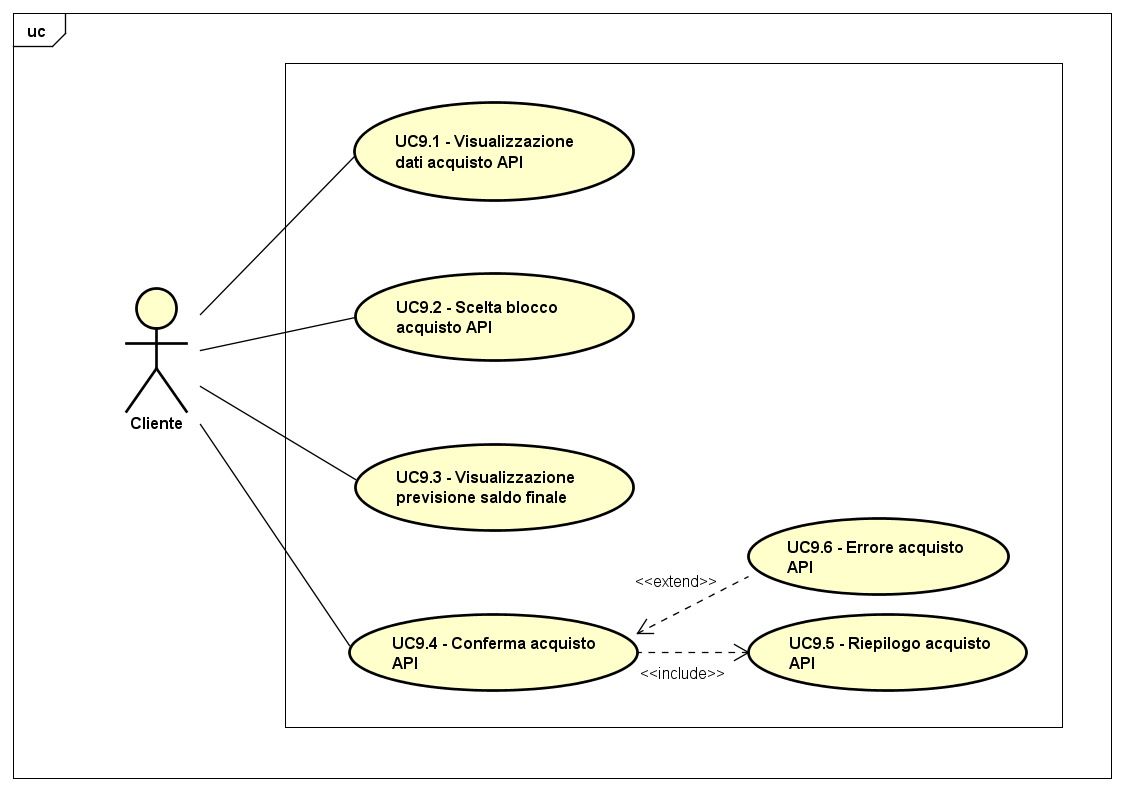
\includegraphics[scale=0.45]{UML/UC9.png}
	\caption{UC9: Acquisto API}
\end{figure}

\begin{longtable}{ l | p{11cm}}
	\hline
	\rowcolor{Gray}
	\multicolumn{2}{c}{UC9 - Acquisto API}\\
	\hline
	\textbf{Attori} & Cliente \\
	\textbf{Descrizione} & L'attore effettua l'acquisto dell'API selezionata tramite i crediti da lui posseduti \\
	\textbf{Pre-Condizioni} & L'attore ha selezionato una API. L'applicazione mostra la relativa schermata di acquisto \\
	\textbf{Post-Condizioni} & L'attore ha acquistato l'API selezionata \\
	\textbf{Scenario Principale} & 
	\begin{enumerate*}[label=(\arabic*.),itemjoin={\newline}]
		\item L'attore può visualizzare i dati d'acquisto dell'API (UC9.1)
		\item L'attore può scegliere la licenza API desiderata (UC9.2)
		\item L'attore può visualizzare il saldo preventivato in seguito all'acquisto dell'API con la licenza selezionata (UC9.3)
		\item L'attore può confermare l'acquisto (UC9.4), venendo reindirizzato ad una schermata di riepilogo (UC9.5)
	\end{enumerate*}\\
	\textbf{Scenari Alternativi} & 
	\begin{enumerate*}[label=(\arabic*.),itemjoin={\newline}]
		\item L'attore può visualizzare un messaggio di errore (E.g: saldo non sufficiente) e la transazione non avviene (UC9.6)
		\item L'attore può scegliere la licenza API per numero di chiamate (UC9.2.1)
		\item L'attore può scegliere la licenza API per tempo di utilizzo (UC9.2.2)
		\item L'attore può scegliere la licenza API per traffico (UC9.2.3)
	\end{enumerate*}\\
\end{longtable}

\subsubsection{Caso d'uso UC9.1: Visualizzazione dati acquisto API}
\label{UC9_1}

\begin{minipage}{\linewidth}
	\begin{tabular}{ l | p{11cm}}
		\hline
		\rowcolor{Gray}
		\multicolumn{2}{c}{UC9.1 - Visualizzazione dati acquisto API} \\
		\hline
		\textbf{Attori} & Cliente \\
		\textbf{Descrizione} & L'attore visualizza i dati d'acquisto dell'API \\
		\textbf{Pre-Condizioni} & L'attore si trova nella schermata di acquisto dell'API \\
		\textbf{Post-Condizioni} & L'attore ha visualizzato i dati d'acquisto dell'API \\
		\textbf{Scenario Principale} & 
		\begin{enumerate*}[label=(\arabic*.),itemjoin={\newline}]
			\item L'attore può visualizzare il nome dell'API (UC9.1.1)
			\item L'attore può visualizzare l'autore dell'API (UC9.1.2)
		\end{enumerate*}\\
	\end{tabular}
\end{minipage}

\paragraph{Caso d'uso UC9.1.1: Visualizzazione nome API}
\label{UC9_1_1}

\begin{minipage}{\linewidth}
	\begin{tabular}{ l | p{11cm}}
		\hline
		\rowcolor{Gray}
		\multicolumn{2}{c}{UC9.1.1 - Visualizzazione nome API} \\
		\hline
		\textbf{Attori} & Cliente \\
		\textbf{Descrizione} & L'attore visualizza il nome dell'API \\
		\textbf{Pre-Condizioni} & L'attore si trova nella schermata di acquisto dell'API \\
		\textbf{Post-Condizioni} & L'attore ha visualizzato il nome dell'API \\
		\textbf{Scenario Principale} & 
		\begin{enumerate*}[label=(\arabic*.),itemjoin={\newline}]
			\item L'attore può visualizzare il nome dell'API
		\end{enumerate*}\\
	\end{tabular}
\end{minipage}

\paragraph{Caso d'uso UC9.1.2: Visualizzazione autore API}
\label{UC9_1_2}

\begin{minipage}{\linewidth}
	\begin{tabular}{ l | p{11cm}}
		\hline
		\rowcolor{Gray}
		\multicolumn{2}{c}{UC9.1.2 - Visualizzazione autore API} \\
		\hline
		\textbf{Attori} & Cliente \\
		\textbf{Descrizione} & L'attore visualizza l'autore dell'API \\
		\textbf{Pre-Condizioni} & L'attore si trova nella schermata di acquisto dell'API \\
		\textbf{Post-Condizioni} & L'attore ha visualizzato l'autore dell'API \\
		\textbf{Scenario Principale} & 
		\begin{enumerate*}[label=(\arabic*.),itemjoin={\newline}]
			\item L'attore può visualizzare l'autore dell'API
		\end{enumerate*}\\
	\end{tabular}
\end{minipage}

\paragraph{Caso d'uso UC9.1.3: Visualizzazione policy vendita API}
\label{UC9_1_3}

\begin{minipage}{\linewidth}
	\begin{tabular}{ l | p{11cm}}
		\hline
		\rowcolor{Gray}
		\multicolumn{2}{c}{UC9.1.3 - Visualizzazione policy vendita API} \\
		\hline
		\textbf{Attori} & Cliente \\
		\textbf{Descrizione} & L'attore visualizza la policy di vendita dell'API \\
		\textbf{Pre-Condizioni} & L'attore si trova nella schermata di acquisto dell'API \\
		\textbf{Post-Condizioni} & L'attore ha visualizzato la policy di vendita dell'API \\
		\textbf{Scenario Principale} & 
		\begin{enumerate*}[label=(\arabic*.),itemjoin={\newline}]
			\item L'attore può visualizzare la policy di vendita dell'API
		\end{enumerate*}\\
	\end{tabular}
\end{minipage}

\subsubsection{Caso d'uso UC9.2: Scelta blocco acquisto API}
\label{UC9_2}

\begin{minipage}{\linewidth}
	\begin{tabular}{ l | p{11cm}}
		\hline
		\rowcolor{Gray}
		\multicolumn{2}{c}{UC9.2 - Scelta blocco acquisto API} \\
		\hline
		\textbf{Attori} & Cliente \\
		\textbf{Descrizione} & L'attore sceglie il blocco da acquistare in base alla policy di vendita dell'API \\
		\textbf{Pre-Condizioni} & L'attore ha selezionato una API e si trova nella relativa schermata di acquisto \\
		\textbf{Post-Condizioni} & L'attore ha scelto il blocco da acquistare in base alla policy di vendita dell'API \\
		\textbf{Scenario Principale} & 
		\begin{enumerate*}[label=(\arabic*.),itemjoin={\newline}]
			\item L'attore può scegliere il blocco da acquistare in base alla policy di vendita dell'API
		\end{enumerate*}\\
	\end{tabular}
\end{minipage}

\subsubsection{Caso d'uso UC9.3: Visualizzazione previsione saldo finale}
\label{UC9_3}

\begin{minipage}{\linewidth}
	\begin{tabular}{ l | p{11cm}}
		\hline
		\rowcolor{Gray}
		\multicolumn{2}{c}{UC9.3 - Visualizzazione previsione saldo finale} \\
		\hline
		\textbf{Attori} & Cliente \\
		\textbf{Descrizione} & L'attore visualizza una previsione del proprio saldo crediti in seguito all'acquisto \\
		\textbf{Pre-Condizioni} & L'attore ha selezionato una API e si trova nella relativa schermata di acquisto \\
		\textbf{Post-Condizioni} & L'attore ha visualizzato una previsione del proprio saldo in seguito all'acquisto \\
		\textbf{Scenario Principale} & 
		\begin{enumerate*}[label=(\arabic*.),itemjoin={\newline}]
			\item L'attore può visualizzare una previsione del proprio saldo finale qualora acquistasse l'API con il blocco di acquisto scelto in UC9.2
		\end{enumerate*}\\
	\end{tabular}
\end{minipage}

\subsubsection{Caso d'uso UC9.4: Conferma acquisto API}
\label{UC9_4}

\begin{minipage}{\linewidth}
	\begin{tabular}{ l | p{11cm}}
		\hline
		\rowcolor{Gray}
		\multicolumn{2}{c}{UC9.4 - Conferma acquisto API} \\
		\hline
		\textbf{Attori} & Cliente \\
		\textbf{Descrizione} & L'attore può confermare l'acquisto dell'API, portando a termine la transazione, ricevendo un'email di riepilogo e visualizzando una schermata di riepilogo dell'acquisto appena realizzato \\
		\textbf{Pre-Condizioni} & L'attore ha selezionato una API e si trova nella relativa schermata di acquisto \\
		\textbf{Post-Condizioni} & L'attore ha confermato l'acquisto dell'API \\
		\textbf{Scenario Principale} & 
		\begin{enumerate*}[label=(\arabic*.),itemjoin={\newline}]
			\item L'attore può confermare l'acquisto dell'API, portando a termine la transazione, ricevendo un'email di riepilogo e visualizzando una schermata di riepilogo dell'acquisto appena realizzato (UC9.5)
		\end{enumerate*}\\
	\end{tabular}
\end{minipage}

\newpage
\subsubsection{Caso d'uso UC9.5: Riepilogo acquisto API}
\label{UC9_5}
\begin{figure}[ht]
	\centering
	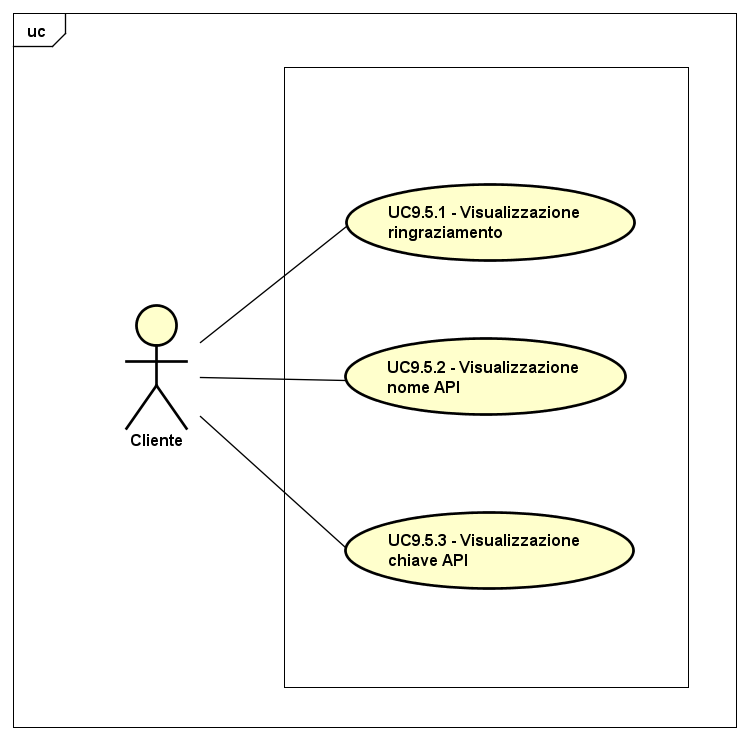
\includegraphics[scale=0.45]{UML/UC9_5.png}
	\caption{UC9.5: Riepilogo acquisto API}
\end{figure}

\begin{minipage}{\linewidth}
	\begin{tabular}{ l | p{11cm}}
		\hline
		\rowcolor{Gray}
		\multicolumn{2}{c}{UC9.5 - Riepilogo acquisto API} \\
		\hline
		\textbf{Attori} & Cliente \\
		\textbf{Descrizione} & L'attore conferma l'acquisto dell'API, portando a termine la transazione e visualizzando un messaggio di ringraziamento \\
		\textbf{Pre-Condizioni} & L'attore ha confermato l'acquisto per l'API \\
		\textbf{Post-Condizioni} & L'attore ha visualizzato il riepilogo dell'acquisto appena realizzato \\
		\textbf{Scenario Principale} & 
		\begin{enumerate*}[label=(\arabic*.),itemjoin={\newline}]
			\item L'attore può visualizzare un messaggio di ringraziamento (UC9.5.1)
			\item L'attore può visualizzare il nome dell'API appena acquistata (UC9.5.2)
			\item L'attore può visualizzare la chiave dell'API appena acquistata (UC9.5.3)
		\end{enumerate*}\\
	\end{tabular}
\end{minipage}

\paragraph{Caso d'uso UC9.5.1: Visualizzazione ringraziamento}
\label{UC9_5_1}

\begin{minipage}{\linewidth}
	\begin{tabular}{ l | p{11cm}}
		\hline
		\rowcolor{Gray}
		\multicolumn{2}{c}{UC9.5.1 - Visualizzazione ringraziamento} \\
		\hline
		\textbf{Attori} & Cliente \\
		\textbf{Descrizione} & L'attore visualizza un messaggio di ringraziamento \\
		\textbf{Pre-Condizioni} & L'attore si trova nella schermata di riepilogo acquisto dell'API \\
		\textbf{Post-Condizioni} & L'attore ha visualizzato un messaggio di ringraziamento \\
		\textbf{Scenario Principale} & 
		\begin{enumerate*}[label=(\arabic*.),itemjoin={\newline}]
			\item L'attore può visualizzare un messaggio di ringraziamento
		\end{enumerate*}\\
	\end{tabular}
\end{minipage}

\paragraph{Caso d'uso UC9.5.2: Visualizzazione nome API acquistata}
\label{UC9_5_2}

\begin{minipage}{\linewidth}
	\begin{tabular}{ l | p{11cm}}
		\hline
		\rowcolor{Gray}
		\multicolumn{2}{c}{UC9.5.2 - Visualizzazione nome API acquistata} \\
		\hline
		\textbf{Attori} & Cliente \\
		\textbf{Descrizione} & L'attore visualizza il nome dell'API acquistata \\
		\textbf{Pre-Condizioni} & L'attore si trova nella schermata di riepilogo acquisto dell'API \\
		\textbf{Post-Condizioni} & L'attore ha visualizzato il nome dell'API acquistata \\
		\textbf{Scenario Principale} & 
		\begin{enumerate*}[label=(\arabic*.),itemjoin={\newline}]
			\item L'attore può visualizzare il nome dell'API acquistata
		\end{enumerate*}\\
	\end{tabular}
\end{minipage}

\paragraph{Caso d'uso UC9.5.3: Visualizzazione chiave API acquistata}
\label{UC9_5_3}

\begin{minipage}{\linewidth}
	\begin{tabular}{ l | p{11cm}}
		\hline
		\rowcolor{Gray}
		\multicolumn{2}{c}{UC9.5.3 - Visualizzazione chiave API acquistata} \\
		\hline
		\textbf{Attori} & Cliente \\
		\textbf{Descrizione} & L'attore visualizza la chiave dell'API acquistata \\
		\textbf{Pre-Condizioni} & L'attore si trova nella schermata di riepilogo acquisto dell'API \\
		\textbf{Post-Condizioni} & L'attore ha visualizzato la chiave dell'API acquistata \\
		\textbf{Scenario Principale} & 
		\begin{enumerate*}[label=(\arabic*.),itemjoin={\newline}]
			\item L'attore può visualizzare la chiave dell'API acquistata
		\end{enumerate*}\\
	\end{tabular}
\end{minipage}

\subsubsection{Caso d'uso UC9.6: Errore acquisto API}
\label{UC9_6}

\begin{minipage}{\linewidth}
	\begin{tabular}{ l | p{11cm}}
		\hline
		\rowcolor{Gray}
		\multicolumn{2}{c}{UC9.6 - Errore acquisto API} \\
		\hline
		\textbf{Attori} & Cliente \\
		\textbf{Descrizione} & L'attore visualizza un messaggio di errore e la transazione non avviene \\
		\textbf{Pre-Condizioni} & L'attore ha confermato l'acquisto per una API ma si è verificato un errore \\
		\textbf{Post-Condizioni} & L'attore ha visualizzato un errore relativo all'acquisto, con opportuna descrizione \\
		\textbf{Scenario Principale} & 
		\begin{enumerate*}[label=(\arabic*.),itemjoin={\newline}]
			\item L'attore può visualizzare un messaggio di errore e la transazione non avviene (E.g: L'API è sospesa)
		\end{enumerate*}\\
	\end{tabular}
\end{minipage}